\section{SPI Unit}

The \gls{SPI} unit provides access to one of the microcontroller's \gls{SPI} peripherals. The unit can be configured to any of the hardware-supported speeds, clock polarity, and clock phase settings. Explanation of those options, including diagrams, can be found in \cref{sec:theory_spi}.

The unit handles up to 16 slave select (\gls{NSS}) signals and supports message multi-cast (addressing more than one slaves at once). Protection resistors should be used if a multi-cast transaction is issued with \gls{MISO} connected to prevent a short circuit between slaves transmitting the opposite logical level.

The QUERY command of this unit, illustrated by \cref{fig:spi_query}, is flexible enough to support all types of \gls{SPI} transactions: read-only, write-only, and read-write, with different request and response lengths and paddings. The slave select signal is asserted during the entire transaction.

\begin{figure}[h]
	\centering
	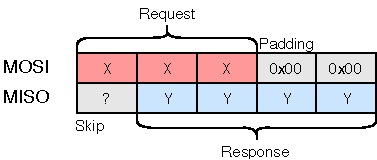
\includegraphics[scale=1.1] {img/spi-query.pdf}
	\caption{\label{fig:spi_query}SPI transaction using the QUERY command}
\end{figure}

\subsection{SPI Configuration}

\begin{inicode}
[SPI:spi@5]
# Peripheral number (SPIx)
device=1
# Pin mappings (SCK,MISO,MOSI)
#  SPI1: (0) A5,A6,A7     (1) B3,B4,B5
#  SPI2: (0) B13,B14,B15
remap=0
# Prescaller: 2,4,8,...,256
prescaller=64
# Clock polarity: 0,1 (clock idle level)
cpol=0
# Clock phase: 0,1 (active edge, 0-first, 1-second)
cpha=0
# Transmit only, disable MISO
tx-only=N
# Bit order (LSB or MSB first)
first-bit=MSB
# SS port name
port=A
# SS pins (comma separated, supports ranges)
pins=0
\end{inicode}

\subsection{SPI Commands}

\begin{cmdlist}
	0 & \cname{QUERY}
	Exchange bytes with a slave device; see the diagram in \cref{fig:spi_query}
	& \begin{cmdreq}
		\cfield{u8} slave number 0--16
		\cfield{u16} response padding
		\cfield{u16} response length
		\cfield{u8[]} bytes to write
	    \end{cmdreq}
	\cjoin
    	\begin{cmdresp}
		\cfield{u8[]} received bytes
	\end{cmdresp} \\

	1 & \cname{MULTICAST}
	Send a message to multiple slaves at once. The ``addressed slaves'' word uses the packed pins format (\cref{sec:packedpins}).
	& \begin{cmdreq}
		\cfield{u16} addressed slaves
		\cfield{u8[]} bytes to write
	\end{cmdreq} \\
\end{cmdlist}


